\chapter{Complementi su insiemi e relazioni}

\section{Funzioni}
Una \textbf{funzione} o \textbf{applicazione} tra due insiemi A e B è una legge per cui per ogni elemento del primo insieme esiste uno e un solo elemento del secondo insieme e viene rappresentata:
\begin{center}
    $f : A \rightarrow B \; t.c. \; \forall a \in A \; \exists ! b \in B \; | \; f(a) = b$
\end{center}
$b$ è l'\textbf{immagine} di $a$. \\ \newline
\textbf{Proprietà delle Funzioni}
\begin{enumerate}[nosep]

    \item la funzione si dice \textbf{iniettiva} se vale che:  $\forall a, a' \in A, \; f(a) = f(a') \Rightarrow a = a'$.

    \item la funzione si dice \textbf{suriettiva} sevale che: $\forall b \in B, \exists a \in A \; | \; f(a) = b$.

    \item una funzione $f : A \rightarrow B$ si dice \textbf{biettiva} o \textbf{biunivoca} se è contemporaneamente \textit{iniettiva} e \textit{suriettiva} ovvero se:
        \begin{center}
            \fcolorbox{red}{white}{$\forall b \in B$} $\;$ \fcolorbox{green}{white}{$\exists ! a \in A$} $\; t.c. \; f(a) = b$
        \end{center}
    il \textcolor{red}{box rosso} identifica l'\textbf{iniettività}, mentre il \textcolor{green}{box verde} identifica la \textbf{suriettività}.
\end{enumerate}

\newpage
\section{Insiemi Discreti}
Due insiemi A e B si dicono \textbf{equipotenti} (o con la stessa \textbf{cardinalità}) se:
\begin{center}
    $f : A \rightarrow B, \; f \; biunivoca$
\end{center}
Siccome $f$ è \textbf{biunivoca} avremo che ogni elemento di A avrà \textbf{uno e un solo} elemento di B distinto e B sarà formato da sole immagini di A portando i due insieme ad avere ``lo stesso numero'' di elementi, utilizzeremo come notazione: $\#A = \#B$.
Un insieme A si dice \textbf{finito} se:
\begin{center}
    $\exists n \in \mathbb{N}, \; f : A \rightarrow \mathbb{N}_n, \; f \; biunivoca$
\end{center}
\begin{boxA}
    \begin{minipage}[t]{0.3\textwidth}
        \centering
        $A = \{ \Box, \boxdot, \blacksquare \}$ \\
        $\mathbb{N}_3 = \{1, 2, 3 \}$
    \end{minipage}
    \begin{minipage}[t]{0.6\textwidth}
        \centering
        contando i simboli dell'insieme A si va a creare un'associazione tra gli elementi di A e di $\mathbb{N}_3$
    \end{minipage}
\end{boxA}
In questo caso diremo che la \textbf{cardinalità} di A è \textbf{n}: $\#A = \#\mathbb{N}_n = n$ \\
Un insieme A si dice \textbf{numerabile} se:
\begin{center}
    $\exists f : A \rightarrow \mathbb{N}, \; f \; biunivoca$
\end{center}
In questo caso si dice che A ha cardinalità numerabile e si può rappresentare attraverso la lettera \textbf{aleph} (è la prima lettera dell'alfabeto ebraico): $\#A = \#\mathbb{N} = \aleph_0$ (si ricordi: \textbf{il Paradosso dell'albergo di Hilbert}). \\
Alcuni esempi: 
\begin{enumerate}[nosep]
    \item l'insieme $\mathbb{Z}$ è \textbf{numerabile} ($\#\mathbb{N} = \#\mathbb{Z}$):
        \begin{center}
            $0 \rightarrow 1$ \\
            $1 \rightarrow 2 \;\;\;\; -1 \rightarrow 3$ \\
            $2 \rightarrow 4 \;\;\;\; -2 \rightarrow 5$
        \end{center}
    possiamo quindi mappare i valori \textbf{positivi} dell'insieme $\mathbb{Z}$ sono mappati nei valori \textbf{pari} dell'insieme $\mathbb{N}$ e in maniera complementare i valori \textbf{negativi} dell'insieme $\mathbb{Z}$ sono mappati nei valori \textbf{dispari} dell'insieme $\mathbb{N}$. È quindi possibile verificare la biunivocità dell'applicazione che mappa i valori da $\mathbb{Z}$ a $\mathbb{N}$.
    \item l'insieme dei numeri \textbf{pari} $\mathbb{P}$ può definirsi numerabile, infatti: $\#\mathbb{P} = \#\mathbb{N}$, in questo caso avremo l'applicazione biunivoca del tipo:
        \begin{center}
            $f : \mathbb{P} \rightarrow \mathbb{N} \; | \; \forall p = 2n \in \mathbb{P}, \; f(p) = \frac{1}{2}p = n$
        \end{center}
\end{enumerate}

\begin{boxA}
    Un insieme A si dice \textbf{discreto} se è \textbf{finito} o \textbf{numerabile} (tutti gli insiemi \textit{numerabili} sono infiniti, ma non tutti gli insimi infiniti sono numerabili)
\end{boxA}
\begin{figure}[h]
    \begin{minipage}[t]{0.4\textwidth}
        \centering
        Se A è finito di cardinalità \textbf{n}, i suoi elementi possono essere etichettati con gli elementi di $\mathbb{N}_n$: $A = \{a_1, a_2, ..., a_n\}$
    \end{minipage}
    \begin{minipage}[t]{0.5\textwidth}
        \centering
        Se A è numerabile, gli elementi possono essere ``etichettati'' con gli elementi di $\mathbb{N}$: $A = \{a_1, a_2, ..., a_n, ...\} = \{a_i \; | \; i \in \mathbb{N} \}$
    \end{minipage}
\end{figure}

\bigskip

\textbf{Funzione Caratteristica}: è un'applicazione ce determina se un elemento appartiene o meno ad un sottoinsieme Y di A ($Y \subseteq A$). Quindi diremo che dato un insieme discreto A ed un suo sottoinsieme $Y \subseteq A$ si dice \textbf{funzione caratteristica} di Y la funzione:
\begin{figure}[h]
    \begin{minipage}{0.5\textwidth}
        \centering
        $f_Y : A \rightarrow \{0, 1\} \; \forall a \in A$
    \end{minipage}
    \begin{minipage}{0.5\textwidth}
        \centering
        \begin{math}
            f_Y(a) = 
            \begin{cases}
                1 \;\;\;\; se \; a \in A \\
                0 \;\;\;\; se \; a \notin A
            \end{cases}
        \end{math}
    \end{minipage}
\end{figure} \\
Nel caso in cui A sia un insieme finito avremo che: $\#A = \sum_{a \in A}{f_Y(a)}$. \\
Se A è un insieme discreto, ed $f : A \rightarrow \{0, 1\}$ una applicazione a valori in $\{0, 1\}$, risulta univocamente determinato il sottoinsieme $Y \subseteq A$ tale che $f$ sia una funzione caratteristica di $Y$:
\begin{center}
    $Y = \{a \in A \; | \; f(a) = 1\}$
\end{center}
Un esempio, definiamo $A = \mathbb{N}$ e sia $f : A \rightarrow \{0, 1\}$ definita da una \textbf{funzione caratteristica} del tipo: $n \rightarrow \frac{1 + (-1)^{n}}{2}$. In questo caso la funzione $f$ identifica, a partire dall'insieme $\mathbb{N}$, il sottoinsieme $\mathbb{P}$ dei numeri pari. \\
Utilizzando la \textbf{funzione caratteristica} si può ricavare la seguente proprietà degli insiemi discreti:
\begin{itemize}[nosep]
    \item se A è finito di cardinalità \textit{n}, l'insieme $\mathcal{P}(a)$ delle \textbf{parti di A} è in corrispondenza biunivoca con l'\textbf{insieme delle n-ple} a valori in $\{0, 1\}$.
    \item se A è numerabile, l'insieme $\mathcal{P}(a)$ delle parti di A è in corrispondenza biunivoca con l'\textbf{insieme delle successioni} a valori in $\{0, 1\}$.
\end{itemize}

\subsection{Proprietà 1}
Se X e Y sono insiemi \textbf{finiti}, con $\#X = n, \; \#Y = m$ e con $X \cap Y = \emptyset$, allora $\#(X \cup Y) = n + m$. \\
\textcolor{olive}{\textbf{Dimostrazione}}: per Hp. esistono due funzioni biettive $f : X \rightarrow \mathbb{N}_n$ e $g : Y \rightarrow \mathbb{N}_m$. Per dimostrare la proprietà occorre costruire una funzione biettiva $h : X \cup Y \rightarrow \mathbb{N}_{n + m}$. Possiamo porre $\forall c \in X \cup Y$ come:
\begin{center}
    \begin{math}
        h(c) = 
        \begin{cases}
            f(c) \qquad \;\; se \; c \in X \\
            g(c) + n \; \;\; se \; c \in Y
        \end{cases}
    \end{math}
\end{center}

\subsection{Proprietà 2}
Se X è un insieme \textbf{finito} con $\#X = n$ ed Y è un insieme \textbf{numerabile}, con $X \cap Y = \emptyset$ allora $\#(X \cup Y)$ è \textbf{numerabile}. \\
\textcolor{olive}{\textbf{Dimostrazione}}: per Hp. esistono due funzioni biettive $f : X \rightarrow \mathbb{N}_n$ e $g : Y \rightarrow \mathbb{N}$. Per dimostrare la proprietà occorre costruire una funzione biettiva $h : X \cup Y \rightarrow \mathbb{N}$. Possiamo porre $\forall c \in X \cup Y$ come:
\begin{center}
    \begin{math}
        h(c) = 
        \begin{cases}
            f(c) \qquad \;\; se \; c \in X \\
            g(c) + n \; \;\; se \; c \in Y
        \end{cases}
    \end{math}
\end{center}
\subsection{Proprietà 3}
Se X e Y sono due insiemi \textbf{numerabili}, allora anche $X \cup Y$ è \textbf{numerabile}. \\
\textcolor{olive}{\textbf{Dimostrazione}}: senza perdere di generalità, supponiamo che $X \cap Y = \emptyset$. Per ipotesi esistono due funzioni biettive $f : X \rightarrow \mathbb{N}$ e $g : Y \rightarrow \mathbb{N}$. Per dimostrare la proprietà occorre costruire una funzione biettiva $h : X \cup Y \rightarrow \mathbb{N}$. Ad esempio, $\forall c \in (X \cup Y)$, si può porre:
\begin{center}
    \begin{math}
        h(c) = 
        \begin{cases}
            2f(c) - 1 \quad se \; c \in X \\
            2g(c) \;\;\; \qquad se \; c \in Y
        \end{cases}
    \end{math}
\end{center}

\textbf{Proposizione}: se X è un insieme numerabile e $Y \subseteq X$ allora Y è un insieme \textbf{discreto}.

\subsection{Proprietà 4}
Se $\{A_i \; | \; i \in \mathbb{N}\} = \{A_1, A_2, ..., A_i, ...\}$ è un \textbf{insieme numerabile} di \textbf{insiemi numerabili}, si ha che:
\begin{center}
    $\#(\bigcup_{i \in \mathbb{N}}A_i) = \#\mathbb{N}$
\end{center}
\textcolor{olive}{\textbf{Dimostrazione}}: senza perdere di generalità, supponiamo che gli insiemi siano fra loro \textbf{disgiunto}: $A_i \cap A_j = \emptyset, \; \forall i \in j$. Per dimostrare la tesi, utilizziamo il \textit{procedimento diagonale di \textbf{Cantor}}, enumerando per righe gli elementi di ciascun insieme, dove avremo come primo indice l'identificativo dell'insieme e come secondo indice quello della colonna:

\begin{center}
    \begin{tabular}{ccccccc}
        $A_1$: & \textcolor{red}{$a_{11}$} & \textcolor{blue}{$a_{12}$} & \textcolor{purple}{$a_{13}$} & \textcolor{brown}{...} & \textcolor{green}{$a_{1h}$} & ... \\
        $A_2$: & \textcolor{blue}{$a_{21}$} & \textcolor{purple}{$a_{22}$} & \textcolor{brown}{$a_{23}$} & \textcolor{green}{...} & $a_{2h}$ & ... \\
        $A_3$: & \textcolor{purple}{$a_{31}$} & \textcolor{brown}{$a_{32}$} & \textcolor{green}{$a_{33}$} & ... & $a_{3h}$ & ... \\
        ... & \textcolor{brown}{...} & \textcolor{green}{...} & ... & ... & ... & ... \\
        $A_i$: & \textcolor{green}{$a_{i1}$} & $a_{i2}$ & $a_{i3}$ & ... & $a_{ih}$ & ... \\
        ... & ... & .. & ... & ... & ... & ... \\
    \end{tabular}
\end{center}
Consideriamo le diagonali \textcolor{red}{$D_1=\{a_{11}\}$}, \textcolor{blue}{$D_2=\{a_{21}, a_{12}\}$}, ..., \textcolor{green}{$D_k$}, ..., dove: $D_k = \{a_{ij} \; | \; i + j = k + 1\}$, dove il valore delle $j$ identifica la posizione all'interno della diagonale $D_k$. Notiamo che sono composte da finiti elementi. Per dimostrare che $\#(\bigcup_{i \in \mathbb{N}}A_i)$ è \textbf{numerabile}, occorre costruire una applicazione biunivoca, tale che:
\begin{center}
    $h : \bigcup_{i \in \mathbb{N}_n} A_i \rightarrow \mathbb{N}$
\end{center}
Idealmente, vorremmo etichettare, ogni generico elemento $a_{ij}$ che apparterrà alla $k-esima$ diagonale, in questo modo si creerà l'applicazione \textit{biunivoca}.

\begin{figure}[h]
    \centering
    \begin{minipage}[t]{0.15\textwidth}
        \centering
        $\#D_k = k$
    \end{minipage}
    $\rightarrow$
    \begin{minipage}[t]{0.4\textwidth}
        \centering
        ci serve la somma delle cardinalità delle diagonali precedenti alla diagonale tale che $a_{ij} \in D_k$
    \end{minipage}
    $\rightarrow$
    \begin{minipage}[t]{0.35\textwidth}
        \centering
        $\sum^{i+j-2}_{k=1} \#D_k = \frac{(i + j - 2) \cdot (i + j - 1)}{2}$
    \end{minipage}
\end{figure}
In questo modo abbiamo ``etichettato'' tutti gli elementi appartenenti alle diagonali precedenti alla diagonale di riferimento $D_k$, ora ci mancano da ``etichettare'' gli elementi che precendo $a_{ij}$ sulla diagonale, ma sapendo che $a_{ij}$ è il \textbf{j-esimo} elemento allora basterà:
\begin{center}
    $h(a_{ij}) = j + \frac{(i + j - 2)(i + j - 1)}{2}$
\end{center}
In questo modo abbiamo ``etichettato'' anche tutti gli elementi che precedono il nostro $a_{ij}$, ma in direttamente abbiamo descritto un'applicazione \textbf{biunivoca} tra $\bigcup_{i \in \mathbb{N}_n} A_i$ e $\mathbb{N}$, ovvero $h(a_{ij})$ che quindi ci permette di dimostrare che anche $\bigcup_{i \in \mathbb{N}_n} A_i$ è \textbf{numerabile}.

\textbf{Conseguenze}:
\begin{itemize}[nosep]
    \item $\mathbb{Z}$ è numerabile: $\mathbb{Z} = \mathbb{N} \cup \{0\} \cup \{ -n \; | \; n \in \mathbb{N}\}$.
    \item $\mathbb{N} \times \mathbb{N}$ è numerabile: $\mathbb{N} \times \mathbb{N} = \{(n, m) \; | \; n, m \in \mathbb{N}\} = \bigcup_{n \in \mathbb{N}} \{(n, m) \; | \; m \in \mathbb{N}\}$.
    \item $\mathbb{Q}$ è numerabile.
\end{itemize}


\begin{boxA}
    \textcolor{purple}{\textbf{Off-Topic}}: \\
    \textbf{Paradosso del Grand Hotel di Hilbert}: il paradosso del \textit{Grand Hotel} inventato dal matematico \textit{David Hilbert} per mostrare alcune caratteristiche del concetto di infinito e le differenze fra opzioni con insieme finiti ed infiniti. Hilbert immagina un hotel con infinite stanze, tutte occupate, e afferma che qualsiasi sia il numero di altri ospiti che sopraggiungano, sarà sempre possibile ospitarli tutti, anche se il loro numero è infinito, purché numerabile. \\
    Nel caso semplice, arriva un singolo nuovo ospite. Il furbo albergatore sposterà tutti i clienti nella camera successiva (l'ospite della 1 alla 2, quello della 2 alla 3, etc.); in questo modo, benché l'albergo fosse pieno è comunque, essendo infinito, possibile sistemare il nuovo ospite.
    Un caso meno intuitivo si ha quando arrivano infiniti nuovi ospiti. Sarebbe possibile procedere nel modo visto in precedenza, ma solo scomodando infinite volte gli ospiti (già spazientiti dal precedente spostamento): sostiene allora Hilbert che la soluzione sta semplicemente nello spostare ogni ospite nella stanza con numero doppio rispetto a quello attuale (dalla 1 alla 2, dalla 2 alla 4,etc.), lasciando ai nuovi ospiti tutte le camere con i numeri dispari, che sono essi stessi infiniti, risolvendo dunque il problema. Gli ospiti sono tutti dunque sistemati, benché l'albergo fosse pieno.
\end{boxA}

\section{Confronto tra Cardinalità}
Si dice che un insieme A ha \textbf{cardinalità minore o uguale} ad un insieme B (e si indica con: $\#A \leq \#B$) se: $\exists f : A \rightarrow B, \; f \; è \; iniettiva$. \\
\textbf{Proprietà}:
\begin{itemize}[nosep]
    \item \textbf{riflessività}: $\forall A, \; \#A \leq \#A$.
    \item \textbf{transitività}: $\#A \leq \#B, \; \#B \leq \#C \Rightarrow \#A \leq \#C$.
    \item \textbf{antisimmetria}: $\#A \leq \#B, \; \#B \leq \#A \Rightarrow \#A = \#B$.
    \item \textbf{tricotomia}: $\forall A, B \Rightarrow \#A \leq \#B \; o \; \#B \leq \#A$.
\end{itemize}
La relazione ``$\leq$'' fra cardinalità è una relazione di ordine totale.

\begin{boxA}
    \textcolor{blue}{\textbf{Lemma}}: $A \subseteq B \subseteq C$ con $\#A = \#B \Rightarrow \#A = \#B = \#C$.
\end{boxA}

\newpage
\textbf{Teorema di Cantor-Bernstein-Schroeder}: Se $\exists f : A \rightarrow B, \; f \; iniettiva$ ed $\exists g : B \rightarrow A, \; g \; iniettiva$ allora $\exists h : A \rightarrow B, \; h \; biunivoca$. \\
\textcolor{olive}{\textbf{Dimostrazione}}: poiché $f$ e $g$ sono iniettive se le restriangamo alla loro immagine biunivoca:
\begin{center}
    $\#A = \#f(A) \; con \; f(A) \subseteq B$ \\
    $\#B = \#g(B) \; con \; g(B) \subseteq A$ \\
\end{center}
Avremo:
\begin{center}
    $g(f(A)) \subseteq g(B) \subseteq A \Rightarrow \#g(f(A)) = \#f(A) = \#A$
\end{center}
e per il \textcolor{blue}{lemma} possiamo dire che $\#g(B) = \#A$ e $\#g(B) = \#B$ e quindi avremo che $\#A = \#B$, questo implica che esiste una funzione $h : A \rightarrow B$ biunivoca.

\textbf{Teorema di Cantor}: se $A$ è un insieme \textbf{numerabile} allora $\mathcal{P}(A)$ ha cardinalità \textbf{maggiore} di $A$:
\begin{center}
    $\#A \leq \#\mathcal{P}(A) \; con \; \#A \neq \#\mathcal{P}(A)$
\end{center}
\textcolor{olive}{\textbf{Dimostrazione}}: 
\begin{itemize}[nosep]
    \item dimostriamo per prima cosa che $\#A \leq \#\mathcal{P}(A)$ basta trovare una funzione definita $f : A \rightarrow \mathcal{P}(A)$ che sia \textbf{iniettiva} e non biunivoca.
    \begin{center}
        $f(a) = \{a\}$
    \end{center}
    Utilizziamo una \textbf{dimostrazione per} \textcolor{blue}{\textbf{assurdo}}: sappiamo che $\mathcal{P}(A)$ è in corrispondenza biunivoca con le successioni a valori in $\{0,1\}$; allora se $\mathcal{P}(A)$ fosse numerabile sarebbe possibile elencare tutte le successioni a valori in $\{0,1\}$:
\end{itemize}
\begin{center}
    \begin{tabular}{ccccccc}
        $S_1$: & \textcolor{yellow}{$S_{11}$} & $S_{12}$ & $S_{13}$ & ... & $S_{1n}$ & ... \\
        $S_2$: & $S_{21}$ & \textcolor{green}{$S_{22}$} & $S_{23}$ & ... & $S_{2n}$ & ... \\
        $S_3$: & $S_{31}$ & $S_{32}$ & \textcolor{blue}{$S_{33}$} & ... & $S_{3n}$ & ... \\
        ... & ... & ... & ... & ... & ... & ... \\
        $S_j$ & $S_{j1}$ & $S_{j2}$ & $S_{j3}$ & ... & $S_{jn}$ & ... \\
        ... & ... & ... & ... & ... & ... & ... \\
    \end{tabular}
\end{center}
Consideriamo la successione a valori in $\{0, 1\}$:

{\centering
    $\bar{S} = \textcolor{yellow}{\bar{S_1}}, \; \textcolor{green}{\bar{S_2}}, \; \textcolor{blue}{\bar{S_3}}, \; ..., \; \bar{S_j}, \; ...$ || dove $\bar{S_j} \neq S_{jj}$ \\
    siccome valori in $\{0,1\}$ se $\bar{S}_j$ è 0 diventerà 1 e viceversa
\par}

\newpage
In questo modo la successione $\bar{S}$ non coincide con nessuna delle successioni $s_j, \; \forall j \in \mathbb{N}$, poiché differisce dalla j-esima successione nel j-esimo elemento e quindi arriviamo ad un \textbf{assurdo}.
Quindi l'insieme delle successioni a valori in $\{0, 1\}$  non può essere numerabile e, quindi, \textbf{non} è \textbf{numerabile} nemmeno $\mathcal{P}(A)$. \\ \newline
\textbf{La Cardinalità di $\mathbb{R}$}: anche $\mathbb{R}$ \textbf{non} è \textbf{numerabile}, infatti: $\#\mathbb{R} = \# ]0,1[$, consideriamo un'applicazione biunivoca tale che $f : \mathbb{R} \rightarrow ]0,1[$, ad esempio:
\begin{center}
    $f(x) = \frac{x}{ |x| + 1 } \; \forall x \in \mathbb{R}$
\end{center}
che stabilisce biunivocità tra $\mathbb{R}$ e $] -1, 1[$ possiamo affermare che $\#\mathcal{P}(\mathbb{N}) = \#]0,1[$, infatti considerando $\forall x \in ]0, 1[$ come la rappresentazione binaria (con virgola) di $x$; se $\epsilon_n$ è l'n-esima cifra dopo la virgola di tale sviluppo $(\epsilon_1, \epsilon_2, ..., \epsilon_n, ...)$ è una successioni a valori in $\{0, 1\}$ quindi
\begin{center}
    $0,\bar{9} = 1 \in \mathbb{R}$ || viene a perdersi la biunivocità \\
    $\Rightarrow \#\mathbb{R} = \# \mathcal{P}(\mathbb{N})$
\end{center}
Questa tipologia di cardinalità viene definita \textbf{cardinalità del continuo} e si denota con \textbf{c} o con $2^{\aleph_0}$.
\begin{boxA}
    \centering
    \textbf{Congettura} (\textit{ipotesi del continuo}) \\ 
    non esistono cardinalità comprese fra $\#\mathbb{N}$ e $\#\mathbb{R} $.
\end{boxA}
\begin{boxA}
    \centering
    \textbf{Congettura} (\textit{ipotesi generalizzata del continuo}) \\
    non esistono cardinalità comprese tra $\#X$ e $\mathcal{P}(X) = 2^{\#X} \; \forall X$ di cardinalità non finita.
\end{boxA}

\section{Relazioni di Equivalenza}
Una \textbf{relazione} $\mathcal{R}$ tra due insiemi A e B è un \textbf{sottoinsieme} del \textbf{prodotto cartesiano} fra A e B, ovvero $\mathcal{R} \subseteq A \times B$.
\begin{boxA}
    \textcolor{orange}{\textbf{Esempio}} \\
    $\mathcal{R} = '\leq'$ è relazione tra i due insiemi $A = \mathbb{N}$ e $B = \mathbb{N}$, poiché definisce un sottoinsieme del prodotto cartesiamo $\mathbb{N} \times \mathbb{N}$. \\
    Ad esempio: $(1, 2) \in \mathcal{R} \; \text{e} \; (2, 1) \notin \mathcal{R}$.
\end{boxA}

Una relazione $\mathcal{R}$ su A si dice \textbf{relazione di equivalenza} se sono vere le seguenti proprietà:
\begin{itemize}[nosep]
    \item \textit{riflessività}: $\forall a \in A \Rightarrow a\mathcal{R}a$
    \item \textit{simmetria}: $\forall a,b \in A \; : \; a\mathcal{R}b \Rightarrow b\mathcal{R}a$
    \item \textit{transitività}: $\forall a,b,c \in A \; : \; a\mathcal{R}b \; e \; b\mathcal{R}c \Rightarrow a\mathcal{R}c$
\end{itemize}
\textbf{Definizione}: sia $\mathcal{R}$ una \textbf{relazione di equivalenza} su A. Per ogni $a \in A$ si dice \textcolor{red}{\textbf{classe di equivalenza}} $[a] = \{x \in A \; | \; x\mathcal{R}a\}$. \\ \newline
\textbf{Proprietà}:
\begin{itemize}[nosep]
    \item $\forall a \in A, \; a \in [a]$ \\
          \textcolor{olive}{\textbf{Dimostrazione}}: è conseguenza diretta della proprietà riflessiva.
    \item $\forall a,b \in A, \; a \in [b] \Rightarrow [b] = [a]$ \\
          \textcolor{olive}{\textbf{Dimostrazione}}: poiché $a \in [b], \; a\mathcal{R}b$. Se $x \in A, \; x \in [a]$, allora $x\mathcal{R}a$; per la \textbf{proprietà transitiva} segue $x\mathcal{R}b$ ovvero $x \in [b]$. Resta così dimostrato che $[a] \subseteq [b]$. Analogamente, se $y \in A, \; y \in [b]$, allora $y\mathcal{R}b$ per la \textbf{proprietà di simmetria}, $a\mathcal{R}b \Rightarrow b\mathcal{R}a$, per cui la transitività assicura $y\mathcal{R}a$, ovvero $y \in [a]$. Resta così dimostrato che $[b] \subseteq [a]$ e quindi $[b] = [a]$.
    \item $\forall a,b \in A, \; [a] = [b] \; oppure \; [a] \cap [b] \neq \emptyset$ \\
          \textcolor{olive}{\textbf{Dimostrazione}}: se $\exists c \in [a] \cap [b]$, si ha $c \in [a]$ e $c \in [b]$, ovvero $c\mathcal{R}a$ e $c\mathcal{R}b$. Applicando la \textbf{proprietà di simmetria} a $c\mathcal{R}a$ si ottiene $a\mathcal{R}c$, per cui la proprietà \textbf{transitiva} assicura $a\mathcal{R}b$, ovvero $a \in [b]$. La seconda proprietà implica $[a] = [b]$. Quindi, se due classi hanno un elemento in comune, le due classi coincidono.
\end{itemize}
\textbf{Insieme Quoziente}: sia A un insieme ed $\mathcal{R}$ una relazione di equivalenza su A. Si definisce \textbf{insieme quoziente} di A rispetto ad $\mathcal{R}$,
\begin{center}
    $\frac{A}{\mathcal{R}} = \{[a] \; | \; a \in A\}$
\end{center}
\textbf{Rappresentante di una classe d'equivalenza}: sia A un insieme ed $\mathcal{R}$ una relazione di equivalenza su A. Ogni elemento $x \in [a]$, si dice \textbf{Rappresentante} di $[a] \in \frac{A}{\mathcal{R}}$. \\
Sia $\mathcal{R}$ la relazione di equivalenza su $\mathbb{R}$ definita da:
\begin{center}
    $(a, b) \in \mathbb{R}$ se e solo se $a - b \in \mathbb{Z}$
\end{center}
L'insieme quoziente $\frac{\mathbb{R}}{\mathcal{R}}$ è in corrispondenza biunivoca con $[0, 1[$: ogni classe può infatti avere come rappresentante significativo il suo unico elemento nell'intervallo $[0, 1[$.

\begin{boxA}
    \textcolor{orange}{\textbf{Esempio}}: sia $\mathcal{R}$ la \textbf{relazione di equivalenza} su $\mathbb{N}_0 \times \mathbb{N}_0$ definita da:
    \begin{center}
        $(a,b)\mathcal{R}(a',b')$ se e solo se $a+b' = a'+b$
    \end{center}
    In generale:
    \begin{itemize}[nosep]
        \item se $a=b$, $[(a,b)] = \{(n,n) \; | \; n \in \mathbb{N}\}$
        \item se $a<b$, $[(a,b)] = \{(n,n+b-a) \; | \; n \in \mathbb{N}\}$
        \item se $a>b$, $[(a,b)] = \{n+a-b,n\ \; | \; n \in \mathbb{N}\}$
    \end{itemize}
    Allora l'insieme quoziente $\frac{\mathbb{N}_0 \times \mathbb{N}_0}{\mathcal{R}}$ è in relazione biunivoca con $\mathbb{Z}$.
\end{boxA}

\begin{boxA}
    \textcolor{orange}{\textbf{Esempi}} \\
    Sia $\mathcal{R}$ la relazione di equivalenza su $\mathbb{N}$ definita da $(a, b) \in \mathcal{R}$ se e solo se $(-1)^a = (-1)^b$. L'\textbf{insieme quoziente} è formato da due classi $\frac{\mathbb{N}}{\mathcal{R}} = \{\mathbb{P}, \mathbb{D}\}$ \\ \newline
    Sia $\mathcal{R}$ la relazione di equivalenza su $\mathbb{R}$ definita da $(a, b) \in \mathbb{R}$ se e solo se $\lfloor a \rfloor = \lfloor b \rfloor$. L'\textbf{insieme quoziente} è in corrispondenza biunivoca con $\mathbb{Z}$ (il passaggio da $\mathbb{R}$ a $\frac{\mathbb{R}}{\mathcal{R}}$ è un esempio di \textbf{discretizzazione}): $\frac{\mathbb{R}}{\mathcal{R}} = \{ [ n, n+1[, n \in \mathbb{Z} \}$
\end{boxA}

\section{Congruenza modulo n}
\textbf{Definizione}: fissa un intero $n \in \mathbb{N}$, si definisce una relazione di equivalenza $\equiv_n$ su $\mathbb{Z}$:
\begin{center}
    $x \equiv_n y$ se e solo se $\exists h \in \mathbb{Z} \; | \; y - x = h \cdot n$
\end{center}
Verifichiamo che $\equiv_n$ è una \textbf{relazione di equivalenze}:
\begin{itemize}[nosep]
    \item \textbf{riflessività}: $\forall x \in \mathbb{Z}, \; x \equiv_n x$ è verificato, poiché $x - x = h \cdot n$ considerando $h = 0 \in \mathbb{Z}$.
    \item \textbf{simmetria}: se $x \equiv_n y$, per definizione $\exists h \in \mathbb{Z}$ tale che $y - x = h \cdot n$. Per dimostrare che $y \equiv_n x$ devo trovare un $h' \in \mathbb{Z} \; | \; x-y = h' \cdot n$. Basta prendere $h'=-h$.
    \item \textbf{transitività}: se $x \equiv_n y$ e $y \equiv_n <$, allora $\exists h \in \mathbb{Z} \; | \; y - x = h \cdot n$ ed $\exists k \in \mathbb{Z} \; | \; z - y = k \cdot n$. Sommando membreo a membro, si ottiene $z - x = (h + k) \cdot n$; siccome $h + k \in \mathbb{Z}$ segue che $x \equiv_n z$.
\end{itemize}
\textbf{Insieme delle classi resto modulo n}: l'insieme quoziente $\mathbb{Z}/ \equiv_n$ è detto \textbf{insieme delle classi resto modulo} $n$ ed è indicato con $\mathbb{Z}_n$: $\mathbb{Z}_n = \frac{\mathbb{Z}}{\equiv_n}$. \\
L'insieme delle classi resto modulo $n$ è costituito da: 
\begin{center}
    $\mathbb{Z}_n = \{[0], [1], [2], ..., [n-1]\}$
\end{center}
\textcolor{olive}{\textbf{Dimostrazione}}: Per ogni $x \in \mathbb{Z}$, la divisione euclidea per $n$ assicura che $\exists q,r \in \mathbb{Z}, \; 0 \leq r < n$ tali che $x = q \cdot n + r$, ovvero che $x - r = q \cdot n$. Quindi, $x \equiv_n r$, da cui $[x] = [r]$, con $r \in \{0,1,..., n-1\}$. \\
Occorre provare che le n classi $[0], [1], ..., [n-1]$ sono a due a due disgiunte, ovvero che $\forall r,s \in \mathbb{Z}, \; 0 \leq r < s < n \Rightarrow [r] \neq [s]$. Per \textbf{assurdo} supponiamo $[r] = [s]$, questo significherebbe che che $\exists h \in \mathbb{Z} \; | \; s - r = h \cdot n$. Per ipotesi $s > r$, per cui $0 < s - r < n$; quindi $s - r$ \textbf{non} può essere multiplo intero di $n$.

\begin{boxA}
    \textbf{Divisione euclidea}: $\forall a,b \in \mathbb{Z}, \, b \neq 0 \Rightarrow \exists q,r \in \mathbb{Z}, \; 0 \leq r < |b| \; | \; a = b \cdot q + r$.
\end{boxA}

\begin{figure}[h]
    \centering
    \begin{minipage}[t]{0.45\textwidth}
        \centering
        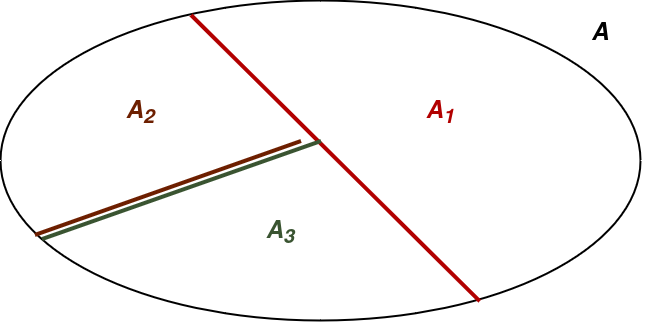
\includegraphics[width=\textwidth]{img/partizionamento}
        \caption{\textbf{Partizionamento}}

        \begin{flushleft}
            Sia A un insieme; un sottoinsieme $\mathcal{B} \subseteq \mathcal{P}(A)$ è detto \textbf{partizione} di A se $\emptyset \notin \mathcal{B}$ e $\forall c \in A, \; \exists ! B \in \mathcal{B} \; | \; x \in B$. Ovvero ogni sottoinsieme non ha intersezione con gli altri.
        \end{flushleft}
    \end{minipage}
    \begin{minipage}[t]{0.45\textwidth}
        \centering
        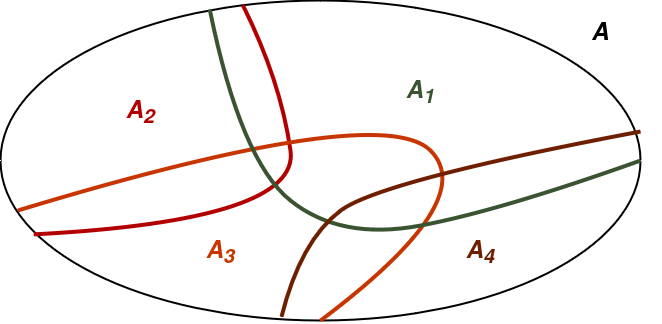
\includegraphics[width=\textwidth]{img/ricoprimento}
        \caption{\textbf{Ricoprimento}}

        \begin{flushleft}
            Sia A un insieme; un sottoinsieme $\mathcal{B} \subseteq \mathcal{P}(A)$ è detto \textbf{ricoprimento} di A se $\forall x \in A, \; \exists B \in \mathcal{B} \; | \; x \in B$.
        \end{flushleft}
    \end{minipage}
\end{figure}

\begin{boxA}
    Se $\mathcal{R}$ è relazione di equivalenza su A, allora l'insieme quoziente $\frac{A}{\mathcal{R}} = \mathcal{B}$ è una partizione di A. 
    Viceversa se $\mathcal{B}$ è una partizione di A, $\exists ! \mathcal{R}$ relazione di equivalenza su A tale che $\frac{A}{\mathcal{R}} = \mathcal{B}$ allora $\mathcal{R}$ è definita da:
    \begin{center}
        $x\mathcal{R}y \Leftrightarrow \exists B \in \mathcal{B} \; | \; x, y \in B$
    \end{center}
\end{boxA}

\begin{boxA}
    \begin{minipage}[t]{0.5\textwidth}
        \centering
        $\mathbb{Z}_4 = \{[0], [1], [2], [3]\}$ \\
    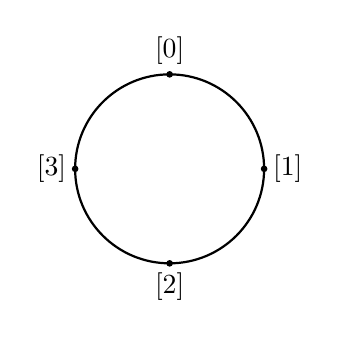
\begin{tikzpicture}[scale=0.6]
        \draw[thick] (0,0) circle(2);
        \foreach \angle/\label in {90/{[0]}, 0/{[1]}, 270/{[2]}, 180/{[3]}} {
            \coordinate (P) at ({2*cos(\angle)},{2*sin(\angle)});
            \fill (P) circle(2pt);
            \node at ({2.5*cos(\angle)},{2.5*sin(\angle)}) {\label};
        }
    \end{tikzpicture}
    \hfill
    \end{minipage}
    \begin{minipage}[t]{0.5\textwidth}
        \centering
    $\mathbb{Z}$ è più facilemente rappresentabile tramite una circonferenza
    \end{minipage}
\end{boxA}